\chapter{Vorauswahl}
Um die möglichen Optionen einzugrenzen, werden im Folgenden die Topologien aufgelistet und die Auswahl anhand einfacher Kriterien eingegrenzt. Einen guten Überblick über Schaltungen für dreiphasige Gleichrichter mit Blindleistungskompensation geben die Präsentationen von Dominik Bortis et al. \cite{Advanced3PhPFC} und Johann W. Kolar \cite{Essenceof3pKolar}. Dabei handelt es sich um Systeme mit aktiver Leistungsfaktorkorrektur. Aufgrund der gewünschten Systemdienstleistungen, wie z.~B. Blindleistungsbereitstellung, sind Systeme mit hybrider Kompensation nicht ausreichend.

\section{Mögliche Topologien}
Die als Vergleichstopologie verwendete ist der bereits im Abschnitt \ref{sec:Rec} vorgestellte dreiphasige Diodengleichrichter. Die anderen Topologien sind nachfolgend aufgeführt.
	\subsection{6-Switch Boost PFC Rectifier}
				Bei der ersten Topologie wurden im Prinzip beim Diodengleichrichter die Dioden durch Schalter ersetzt, siehe Abbildung \ref{fig:sixswitchboost} Dies ermöglicht im Zusammenspiel mit den Eingangsimpedanzen ein Boost-Verhalten und die Modulation der Eingangsströme über verschiedene \gls{PWM}-Verfahren zum gewünschten sinusförmigen Eingangsstrom.
			\begin{figure} 
				\centering
				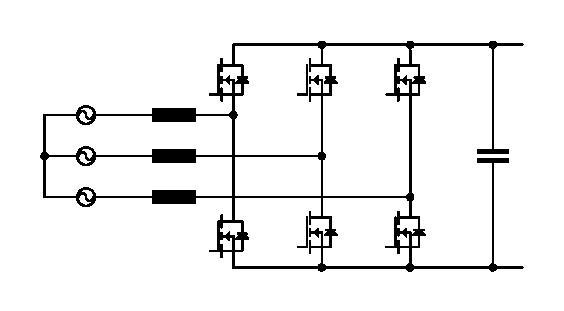
\includegraphics[width=1\linewidth]{content/Grafiken/SixSwitchBoost}
				\caption{Six Switch Boost PFC Rectifier}
				\label{fig:sixswitchboost}
			\end{figure}
		
	\subsection{6-Switch Buck PFC Rectifier}
		\label{sec:6switchBuck}
		Durch das Verschieben der Drossel auf die Ausgangsseite entsteht aus dem 6-Switch Boost eine Tiefstellende Topologie. Allerdings wird ein sperrendes Verhalten in beide Richtungen benötigt, um die Ausgangsspannung und den Eingangsstrom in die gewünschte Form zu bringen. Durch die Schalter wird der Tiefsetzende Strompfad ermöglicht. Aus diesem Grund werden die Schalter durch Dioden ergänzt, wie in Abbildung \ref{fig:sixswitchbuck} dargestellt.  
		
		\begin{figure}
			\centering
			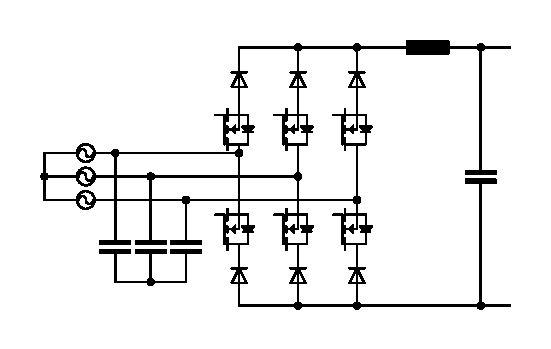
\includegraphics[width=1\linewidth]{content/Grafiken/SixSwitchBuck}
			\caption{Six Switch Buck PFC Rectifier}
			\label{fig:sixswitchbuck}
		\end{figure}
		
		\subsection{Trident Rectifier}
		Diese Topologie basiert auf dem 6-Switch Boost Rectifier. An jeder Phasenhalbbrücke ist ein eigener Tiefsetzsteller angeschlossen. Dadurch besitzt jede Phase einen unabhängigen, identischen parallelen Aufbau zwischen AC- und DC-Pfad (siehe Abbildung \ref{fig:trident}). Dies ermöglicht kontinuierliche Ein- und Ausgangsströme und durch die Wahl des Hoch- oder Tiefsetzenden Strompfades verringern sich die Schaltverluste.
		\begin{figure}
			\centering
			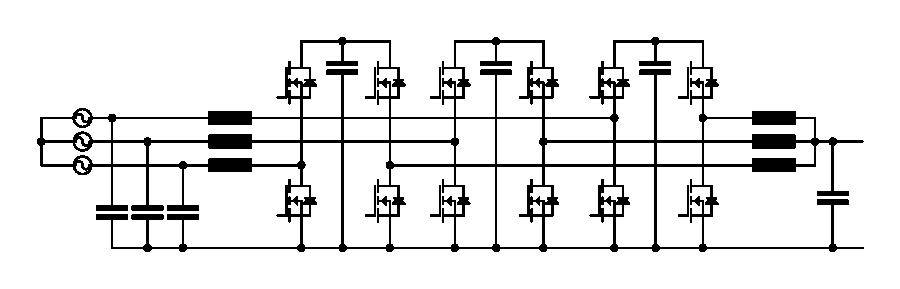
\includegraphics[width=1\linewidth]{content/Grafiken/Trident}
			\caption{Trident Rectifier}
			\label{fig:trident}
		\end{figure}
		
		\subsection{Vienna Rectifier}
		Hierbei handelt es sich ebenfalls um eine hochsetzstellende Topologie. Sie besteht aus einem Diodengleichrichter mit Eingangsinduktivitäten und wird durch einen \gls{IVS} ergänzt, an dem Kapazitäten zur Erzeugung der Ausgangsspannung zugeschaltet werden können. Siehe Abbildung \ref{fig:vienna}. Durch diese 3-Level Struktur kann eine bessere Form des Eingangsstroms erreicht werden als bei der 2-Level 6-Switch Boost PFC Topologie. Durch das weitere Spannungslevel, kann in feineren Stufen geschaltet und somit präziser die gewünschte Stromform eingestellt werden. Außerdem kann aus gleichem Grund die Induktivität kleiner ausfallen.
		\begin{figure}
			\centering
			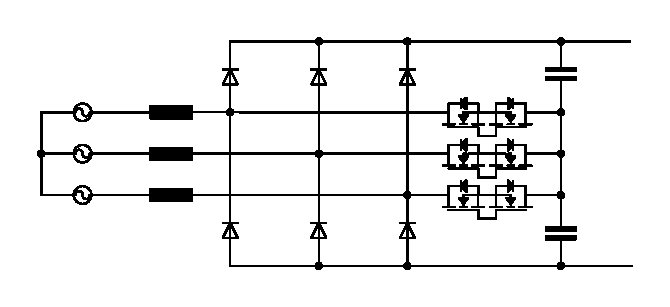
\includegraphics[width=1\linewidth]{content/Grafiken/Vienna}
			\caption{Vienna Rectifier}
			\label{fig:vienna}
		\end{figure}
	
	\subsection{Swiss Rectifier}
		Diese Topologie integriert den Tiefsetzsteller in die Schaltung des \gls{IAF}, siehe Abschnitt \ref{sec:IAF}. Dazu wird die Induktivität im IVS-Pfad mit der des Tiefsetzstellers kombiniert und der Schalter des Tiefsetzstellers durch eine Diode ersetzt. Die Schaltung ist in Abbildung \ref{fig:swiss} zu finden. Durch die Einsparung des Schalters kann die Effizienz gesteigert werden.
		\begin{figure}
			\centering
			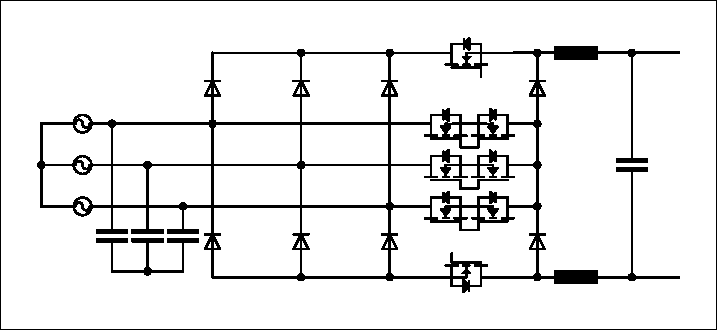
\includegraphics[width=1\linewidth]{content/Grafiken/Swiss}
			\caption{Swiss Rectifier}
			\label{fig:swiss}
		\end{figure}
		
	\subsection{2/3 PWM Buck \& Boost Current Source Rectifier} \label{sec:2/3BuckBoost}
		Um einen größeren Bereich an Ausgangsspannungen abdecken zu können, wird der 6-Switch Buck mit Bidirektionalen Schaltern und durch einen Hochsetzsteller am Ausgang erweitert. Dies zeigt die Abbildung \ref{fig:23pwmbuckboost}. 
		\begin{figure}
			\centering
			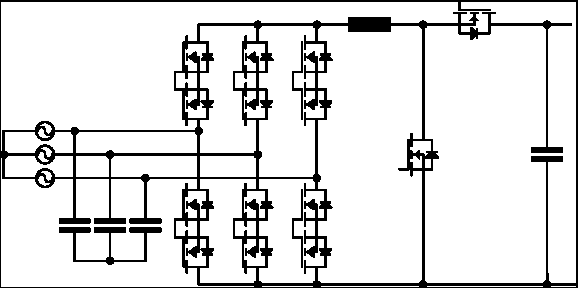
\includegraphics[width=1\linewidth]{content/Grafiken/23PWMBuckBoost}
			\caption{2/3 PWM Buck \& Boost Current Source Rectifier}
			\label{fig:23pwmbuckboost}
		\end{figure}
	
		
	\subsection{Y-Rectifier}
		Anstelle der Topologie aus \ref{sec:2/3BuckBoost} mit Hoch- und Tiefsetzsteller wird hier die umgekehrte Variante mit Tief- und Hochsetzsteller verwendet. Dies ermöglicht kontinuierliche Ein- und Ausgangsspannungen. Außerdem sinken die Schaltverluste, da jeweils nur der Hoch- oder Tiefsetzende Pfad geschaltet wird. Die Schaltung ist in Abbildung \ref{fig:y-rectifier} gezeigt.
		
	
		\begin{figure}
			\centering
			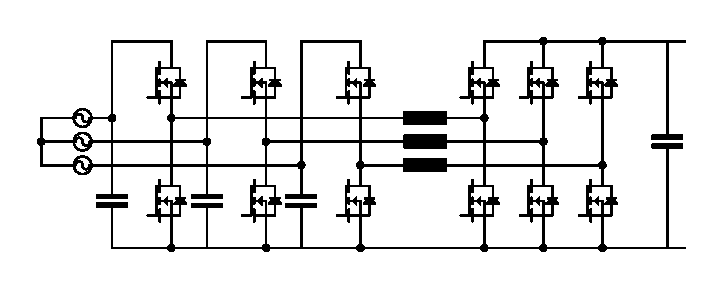
\includegraphics[width=1\linewidth]{content/Grafiken/Y-Rectifier}
			\caption{Y Rectifier}
			\label{fig:y-rectifier}
		\end{figure}
	
	\subsection{3-Level Neutral Point Clamped (NPC)}
		Die 3L-\gls{NPC}-Schaltung ist eine langjährig entwickelte Topologie, die durch verschiedene Ansteuerverfahren unterschiedliche Eigenschaften erzeugt. Unter anderem kann die Reduzierung der Oberschwingungen im Netzstrom und der Rechenaufwand durch optimierte Ansteuerungen verbessert werden \cite{NPC}. Die Schaltung benötigt insgesamt 12 Schalter und 6 Dioden sowie eine dreiphasige Drossel. Der vereinfachte Aufbau der Schaltung ist in Abbildung \ref{fig:3l-npc} dargestellt.
		\begin{figure}
			\centering
			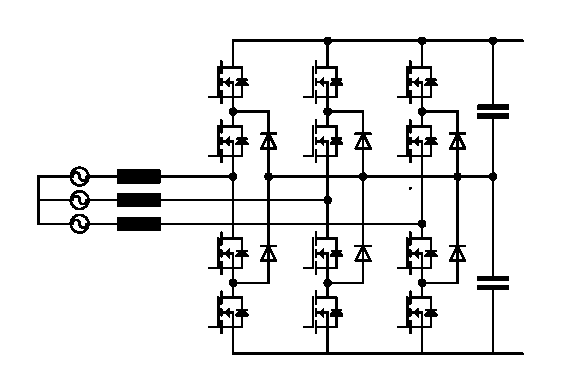
\includegraphics[width=1\linewidth]{content/Grafiken/3L-NPC}
			\caption{3-Level Neutral Point Clamped}
			\label{fig:3l-npc}
		\end{figure}

	\subsection{3-Level Active Neutral Point Clamped (ANPC)}
		Bei der \gls{ANPC}-Schaltung werden die Dioden der \gls{NPC}-Schaltung durch Schalter ersetzt, um den Sternpunkt kontrollieren zu können, siehe Abbildung \ref{fig:anpc}. Auch hier gibt es verschiedene \gls{PWM}-Strategien, die unterschiedliche Schwerpunkte setzen, außerdem ist die Verteilung der Verlustleistung in den Halbleitern nicht trivial \cite{ANPC}.
	
		\begin{figure}
			\centering
			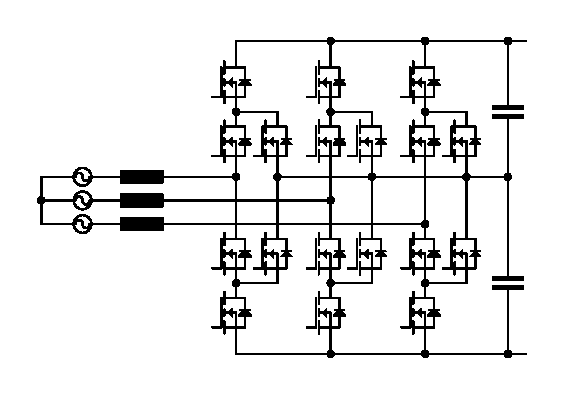
\includegraphics[width=0.9\linewidth]{content/Grafiken/ANPC}
			\caption{3-Level ANPC}
			\label{fig:anpc}
		\end{figure}
	
	
	\subsection{Three-Level Flying Capacitor (FC) Boost-Type Rectifier System}
		Diese Topologie benötigt Kondensatoren für jede Phase, die ein größeres Volumen besitzen, benötigt jedoch weniger Schalter für die drei Level. Die Schaltung ist in Abbildung \ref{fig:3l-fc-boost} dargestellt und besitzt ein hochstellendes Verhalten.
		\begin{figure}
			\centering
			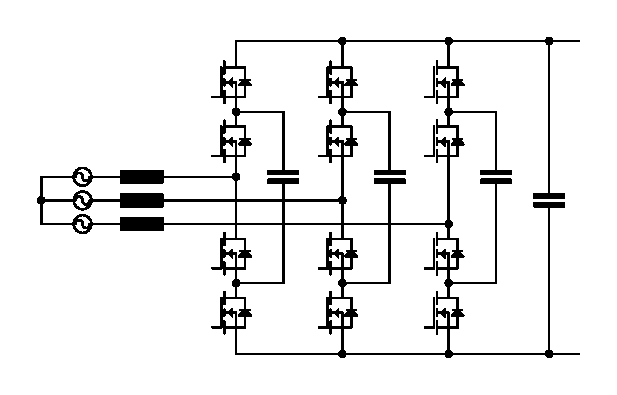
\includegraphics[width=1\linewidth]{content/Grafiken/3L-FC-Boost}
			\caption{Three Level Flying Capacitor Boost-Type}
			\label{fig:3l-fc-boost}
		\end{figure}
	
	
	\subsection{Three-Level Flying Capacitor (FC + Tiefsetzsteller)}
		Um den gewünschten niedrigen Ausgangsspannungsbereich generieren zu können, wird die zuvor beschriebene FC-Topologie durch einen Tiefsetzsteller ergänzt. Dadurch erhöht sich die Anzahl der benötigten Schalter von 12 auf 14.
		\begin{figure}
			\centering
			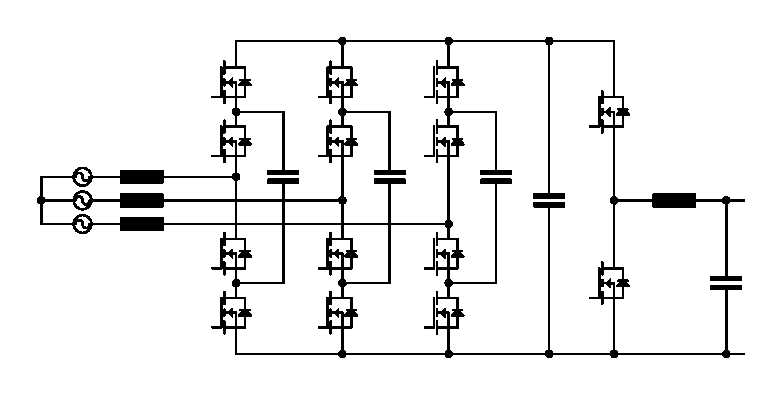
\includegraphics[width=1\linewidth]{content/Grafiken/3L-FC-Boost+Buck}
			\caption{3L FC + Tiefsetzsteller}
			\label{fig:3l-fc-boostbuck}
		\end{figure}

\section{Auswahl der Topologien}
Zur Eingrenzung des Lösungsraums wird zunächst eine Auflistung der möglichen Schaltungstopologien zum Anschluss an das dreiphasige Stromnetz erstellt, vergleiche Tabelle \ref{tab:vorauswahl}. Die 15 aufgelisteten Topologien, beginnend mit dem in Abbildung \ref{fig:B6DiodRect} dargestellten Diodengleichrichter, werden anhand der benötigten Induktivitäten, Dioden, Schalter und Stufen, sowie der Funktionen hoch- bzw. tiefstellend bewertet.\\
Aufgrund ihres simpleren Aufbaus sind Dioden günstiger als Leistungsschalter und fallen daher nicht so stark ins Gewicht. \\
Daher ist der Swiss Rectifier trotz seiner 8 Dioden aber lediglich benötigter 8 Schalter von Interesse. Reine hochsetzende (Boost) Topologien kommen für die Anwendung nicht infrage, da eine niedrige Spannung als Anforderung gestellt wird um den Elektrolyseur hochzufahren. \\
Die Tabelle \ref{tab:vorauswahl} zeigt, dass sich die vier Topologien, die grün hervorgehoben sind, für eine engere Betrachtung eignen, da sie im Vergleich zu anderen Topologien weniger Induktivitäten und Halbleiter benötigen. Die Anzahl der Halbleiter beeinflusst die Kosten und Effizienz der Schaltung und spielen daher eine essentielle Rolle. Anhand der Anzahl an Induktivitäten im Hauptstrompfad wird der Einfluss dieser verglichen. \\
Aufgrund der Komplexität der Schaltungen und benötigten Regelungen werden in dieser Arbeit der \gls{IAF} und \gls{B6PFC} betrachtet und die Ergebnisse für eine finale Bewertung aufbereitet. Die beiden anderen Topologien, 6-Switch Buck und Swiss Rectifier, werden in  der Arbeit von Steffen Isfort betrachtet.

\begin{table}
	\caption{Topologievergleich zur Vorauswahl}
	\label{tab:vorauswahl}
\begin{tabular}{|>{\centering\arraybackslash}p{3cm}|c|c|c|c|c|} %>{\centering\arraybackslash}m{2cm}|>{\centering\arraybackslash}m{2cm} | >{\centering\arraybackslash}m{2cm}|>{\centering\arraybackslash}m{2cm} |>{\centering\arraybackslash}m{2cm}
	& Induktivitäten & Dioden & Schalter & Buck/Boost & Stufen \\
	\hline
	3-ΦDiode Bridge Rectifier & \cellcolor{yellow!25}3 &\cellcolor{red!25}6 &\cellcolor{green!25} 0 & \cellcolor{red!25}- & \cellcolor{green!25}1 \\
	\hline
	6-Switch Boost PFC Rectifier & \cellcolor{yellow!25}3 &\cellcolor{green!25} 0 & \cellcolor{green!25}6 & \cellcolor{red!25}Boost & \cellcolor{green!25}1 \\
	\hline
	Vienna Rectifier & \cellcolor{yellow!25}3 &\cellcolor{red!25}6 & \cellcolor{green!25}6 & \cellcolor{red!25}Boost & \cellcolor{green!25}1 \\
	\hline
	\cellcolor{green!10}6-Switch Buck PFC Rectifier & \cellcolor{green!25}1 &\cellcolor{red!25}6 &\cellcolor{green!25} 6 & \cellcolor{green!25}Buck & \cellcolor{green!25}1 \\
	\hline
	\cellcolor{green!10} \gls{IAF} & \cellcolor{green!25} 2 &\cellcolor{red!25}6 & \cellcolor{yellow!25}10 & \cellcolor{green!25}Buck & \cellcolor{red!25}2 \\
	\hline
	\cellcolor{green!10}Swiss Rectifier & \cellcolor{green!25}1 &\cellcolor{red!25}8 &\cellcolor{green!25} 8 & \cellcolor{green!25} Buck & \cellcolor{red!25}2 \\
	\hline
	\cellcolor{green!10} \gls{B6PFC} &\cellcolor{yellow!25}4 & \cellcolor{green!25} 0 &\cellcolor{green!25} 8 &\cellcolor{green!25} Boost/Buck & \cellcolor{red!25}2 \\
	\hline
	2/3 PWM Buck \& Boost Current Source Rectifier & \cellcolor{green!25} 1 & \cellcolor{green!25}0 & \cellcolor{yellow!25}14 & \cellcolor{green!25}Buck/Boost & \cellcolor{red!25}2 \\
	\hline
	Trident Rectifier & \cellcolor{red!25}6 &\cellcolor{green!25}0 & \cellcolor{yellow!25}12 & \cellcolor{green!25}Buck/Boost & \cellcolor{red!25}2 \\
	\hline
	Y-Rectifier & \cellcolor{yellow!25}3 &\cellcolor{green!25}0 & \cellcolor{yellow!25}12 &\cellcolor{green!25} Buck/Boost & \cellcolor{red!25}2 \\
	\hline
	3-Level Neutral Point Clamped & \cellcolor{yellow!25}3 &\cellcolor{red!25}6 & \cellcolor{yellow!25}12 & \cellcolor{red!25}Boost & \cellcolor{green!25}1 \\
	\hline
	3-Level Active Neutral Point Clamped  & \cellcolor{yellow!25}3 & \cellcolor{green!25}0 & \cellcolor{red!25}18 & \cellcolor{red!25}Boost & \cellcolor{green!25}1 \\
	\hline
	3-Level Active Neutral Point Clamped + Tiefsetzsteller & \cellcolor{yellow!25}4 &\cellcolor{green!25} 0 & \cellcolor{red!25}20 & \cellcolor{green!25}Boost/Buck & \cellcolor{red!25}2 \\
	\hline
	Three-Level Flying Capacitor (FC) Boost-Type Rectifier System & \cellcolor{yellow!25}3 & \cellcolor{green!25}0 & \cellcolor{yellow!25}12 & \cellcolor{red!25}Boost & \cellcolor{green!25}1 \\
	\hline
	Three-Level Flying Capacitor (FC + Tiefsetzsteller) & \cellcolor{yellow!25}4 &\cellcolor{green!25}0 & \cellcolor{yellow!25}14 &\cellcolor{green!25} Boost/Buck &\cellcolor{red!25} 2 \\
\end{tabular}
\end{table}
